\documentclass{article}

\usepackage{fancyhdr}
\usepackage{amsmath}
\allowdisplaybreaks
\usepackage{amsthm}
\usepackage{amsfonts}
\usepackage{tikz}
\usepackage[plain]{algorithm}
\usepackage{algpseudocode}
\usepackage{enumitem}
\usepackage{tikz}
\usepackage{pgfplots}
\pgfplotsset{compat=1.18}
\usepgfplotslibrary{groupplots}
\usepackage{comment}

\usetikzlibrary{automata,positioning}

%
% Basic Document Settings
%

\topmargin=-0.45in
\evensidemargin=0in
\oddsidemargin=0in
\textwidth=6.5in
\textheight=9.0in
\headsep=0.25in

\linespread{1.1}

\pagestyle{fancy}
\lhead{\hmwkAuthorName}
\chead{} % empty
\rhead{\hmwkHeaderTitle}
\cfoot{\thepage}

\renewcommand\headrulewidth{0.4pt}
\renewcommand\footrulewidth{0pt}

\setlength\parindent{0pt}

%
% Homework Details
%

\newcommand{\hmwkTitle}{Homework 2}
\newcommand{\hmwkDueDate}{Monday, January 19, 2026}
\newcommand{\hmwkClass}{ICMA 216 Calculus IIIA}
\newcommand{\hmwkClassTime}{Section 1}
\newcommand{\hmwkClassInstructor}{Ruth J. Skulkhu}
\newcommand{\hmwkAuthorName}{\textbf{Jiraroj Wiruchpongsanon (6781617)}}
\newcommand{\hmwkHeaderTitle}{ICMA 216 Calculus IIIA: Homework 2}

%
% Title Page
%

\title{
    \vspace{2in}
    \textmd{\textbf{\hmwkClass:\ \hmwkTitle}}\\
    \normalsize\vspace{0.1in}\small{Due\ on\ \hmwkDueDate}\\
    \vspace{0.1in}\large{\textit{\hmwkClassInstructor\ \hmwkClassTime}}
    \vspace{3in}
}

\author{\hmwkAuthorName}
\date{}

\renewcommand{\part}[1]{\textbf{\large Part \Alph{partCounter}}\stepcounter{partCounter}\\}

%
% Helper Commands
%

\newcounter{partCounter}
\newcommand{\solution}{\textbf{\large Solution}}

\newtheorem*{theorem}{Theorem}

\theoremstyle{remark}
\newtheorem*{remark}{Remark}

\begin{document}

\maketitle
\newpage

\section*{Problem 1 (11.1 Three dimensional space)}
Find an equation of the sphere that passes through the point $(4,3,-1)$ and has center $(3,8,1)$.

\medskip
\solution

Since we were given two points: $(4, 3, -1)$ and $(3, 8, 1)$, we first find the sphere's radius: 

\[r = \sqrt{(4-3)^2 + (3-8)^2 + (-1-1)^2}\]

we'll get $r = \sqrt{30}$, and now we can shift the sphere's center from the origin to point $(3, 8, 1)$ as \\
\begin{center}
    \boxed{$(x - 3)^2 + (y - 8)^2 + (z - 1)^2  = 30 \hspace{1em}; \hspace{1em} x, y, z \in \mathbb{R}$}
\end{center}    % I"m sorry, this is so ugly

\vspace{1em}
\hrulefill

\section*{Problem 2 (11.1 Three dimensional space)}
Sketch the graph of the following equation in 3-dimensional space.
\begin{enumerate}[label=(\alph*)]
    \item $y = x$
    \item $x^2 + y^2 = 1$
    \item $y = z^2$
\end{enumerate}

\medskip
\solution

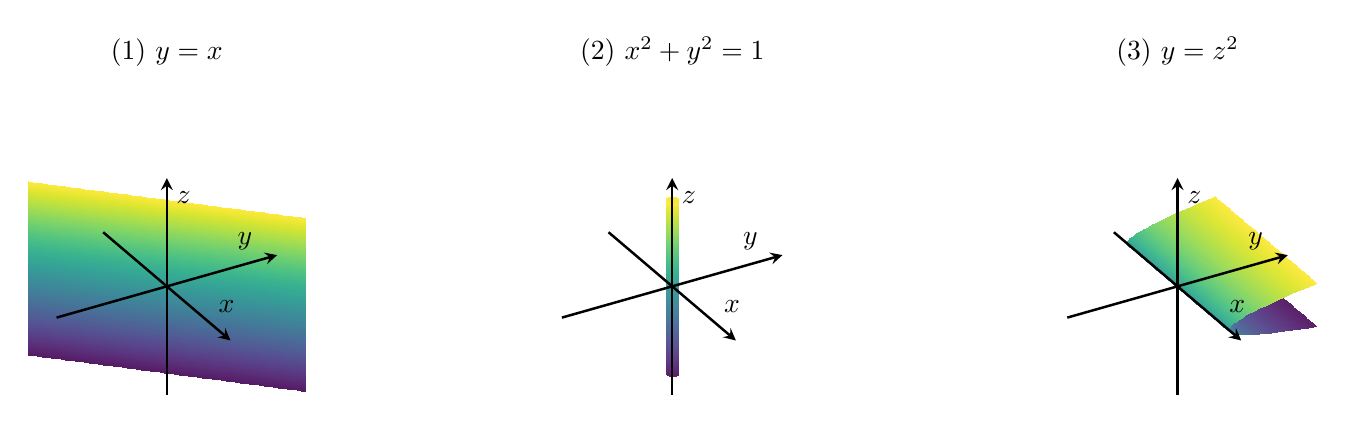
\begin{tikzpicture}
    \begin{groupplot}[
      group style={group size=3 by 1, horizontal sep=2cm},
      width=6cm, height=6.5cm,
      view={60}{30},
      axis lines=center,
      axis line style={line width=0.9pt},
      axis on top,
      ticks=none,
      xlabel={$x$}, ylabel={$y$}, zlabel={$z$},
      xmin=-20, xmax=20,
      ymin=-20, ymax=20,
      zmin=-20, zmax=20,
      colormap/viridis,
    ]
      \nextgroupplot[title={(1)\ $y=x$}]
        \addplot3[
          surf, shader=interp, opacity=0.9,
          domain=-16:16,
          y domain=-16:16,
          samples=60, samples y=40
        ] ({x},{x},{y});

      \nextgroupplot[title={(2)\ $x^{2}+y^{2}=1$}]
        \addplot3[
          surf, shader=interp, opacity=0.88,
          domain=0:2*pi,
          y domain=-16:16,
          samples=120, samples y=40
        ] ({cos(deg(x))},{sin(deg(x))},{y});

      \nextgroupplot[title={(3)\ $y=z^{2}$}]
        \addplot3[
          surf, shader=interp, opacity=0.88,
          domain=-16:16,
          y domain=-4:4,
          samples=80, samples y=40
        ] ({x},{(y)^2},{y});
    \end{groupplot}
  \end{tikzpicture}

\vspace{1em}

\remark I promise I'll plot the graph manually, in real life, later --- when i have access to a piece of paper and a pencil.

\vspace{1em}
\hrulefill

\section*{Problem 3 (11.1 Three dimensional space)}
Let $P_1 = (1,-2,2)$ and $P_2 = (3,4,-12)$ be endpoints of the diameter of a sphere.
\begin{enumerate}[label=(\alph*)]
    \item Find the center and radius of the sphere.
    \item Find the equation of the sphere.
\end{enumerate}

\medskip
\solution

We are given two points: $(1, -2, 2)$ and $(3, 4, -12)$. Firstly, we can find the center point of the sphere by

  \[
  C = \left(\frac{1+3}{2},\frac{-2+4}{2},\frac{2+(-12)}{2}\right) = (2,1,-5)
  \]

So, the center point is at $(1, 3, -7)$; now we find the radius, which is the distance from the sphere's center to any of the two points (I'll do both, as a safety net)

  \begin{align*}
  r &= \sqrt{(1-2)^2 + (-2-1)^2 + (2-(-5))^2} \\
  &= \sqrt{(-1)^2 + (-3)^2 + 7^2}
  = \sqrt{59}, \\
  r &= \sqrt{(3-2)^2 + (4-1)^2 + (-12-(-5))^2} \\
  &= \sqrt{1^2 + 3^2 + (-7)^2}
  = \sqrt{59}.
  \end{align*}

The result are equivalent, and we get the center of the sphere as \boxed{$(2, 1, -5)$} and the redius as \boxed{$\sqrt{59}$}

Now, we can derived the sphere's implicit equation as
    \[
        \boxed{(x - 2)^2 + (y - 1)^2 + (z + 5)^2 = 59}
    \]

\vspace{1em}
\hrulefill

\section*{Problem 4 (11.2 Vectors)}
Let $\mathbf{v} = \mathbf{i} - 2\mathbf{j} + \mathbf{k}$ and $\mathbf{w} = \mathbf{j} + 2\mathbf{k}$. Find
\begin{enumerate}[label=(\alph*)]
    \item $\lVert \mathbf{v} \rVert$,
    \item $3\mathbf{v} - 4\mathbf{w}$,
    \item unit vector of $\mathbf{v} + \mathbf{w}$.
\end{enumerate}

\medskip
\solution

\begin{enumerate}[label=(\alph*)]
    \item $\lVert \mathbf{v} \rVert = \sqrt{1^{2}+(-2)^{2}+1^{2}} = \boxed{\sqrt{6}}$.
    \item $3\mathbf{v}-4\mathbf{w} = 3(\mathbf{i}-2\mathbf{j}+\mathbf{k}) -
  4(\mathbf{j}+2\mathbf{k})
          = \boxed{3\mathbf{i}-10\mathbf{j}-5\mathbf{k}}$.
    \item we first find $\mathbf{v}+\mathbf{w}$
        \[
            \mathbf{v}+\mathbf{w} = (\mathbf{i}-2\mathbf{j}+\mathbf{k}) + (\mathbf{j}+2\mathbf{k})
          = \mathbf{i}-\mathbf{j}+3\mathbf{k}
        \] 
        then it's norm as
          \[
              \lVert \mathbf{v}+\mathbf{w} \rVert = \sqrt{1^{2}+(-1)^{2}+3^{2}} = \sqrt{11}
          \]
          and the unit vector is
          $\displaystyle \frac{\mathbf{v}+\mathbf{w}}{\lVert \mathbf{v}+\mathbf{w} \rVert}
          = \boxed{\frac{1}{\sqrt{11}} \cdot (\mathbf{i}-\mathbf{j}+3\mathbf{k})}$.
  \end{enumerate}

\vspace{1em}
\hrulefill

\section*{problem 5 (11.2 vectors)}
let $\mathbf{u} = \mathbf{i} - 3\mathbf{j} + 5\mathbf{k}$ and $\mathbf{v} = a\mathbf{i} + 12\mathbf{j} + b\mathbf{k}$. find constants $a$ and $b$ that make the vector $\mathbf{u}$ parallels to $\mathbf{v}$.

\medskip
\solution

in order for a vector to be parallel, it's unit vector must be equivalent. the unit vector of $\mathbf{u}$ is

\[
  \widehat{\mathbf{u}}
  = \frac{1}{\sqrt{1^2+(-3)^2+5^2}} \cdot (\mathbf{i}-3\mathbf{j}+5\mathbf{k})
  = \frac{1}{\sqrt{35}} \cdot (\mathbf{i}-3\mathbf{j}+5\mathbf{k}).
\]

  \[
  \widehat{\mathbf{v}}
  = \frac{1}{\sqrt{a^{2}+12^{2}+b^{2}}} \cdot (a\mathbf{i}+12\mathbf{j}+b\mathbf{k})
  \]

\[
  \widehat{\mathbf{v}}
  = \frac{4}{\sqrt{a^{2}+12^{2}+b^{2}}} \cdot (\frac{a}{4}\mathbf{i}+3\mathbf{j}+\frac{b}{4}\mathbf{k})
\]

\vspace{1em}

Compare the direction vector of \mathbf{v} to the direction vector of \mathbf{u}, we'll get \boxed{$a = 4$} and \boxed{$b = 20$} --- which we don't care about the leading scalar. 

\vspace{1em}
\hrulefill

\end{document}
